\chapter[TP1]{\uline{TP1}}
\section[R\`esolution num\'erique de l`\'equation de transport]{\uline{R\`esolution num\'erique de l`\'equation de transport:}}

Soit $c>0$ et le probl\`eme de tranport suivant:

\begin{equation}
\label{systeme}
\left \lbrace \begin{array}{rl}
\partial_t u + c \partial_x u= 0, & \quad x \in ]0,L[, \; t \in ]0,T[, \\
u(0,t) = e^{-t}, & \; t \in ]0,T[, \\
u(x,0) = 0, & \; x \in ]0,L[,
\end{array}\right.
\end{equation}

\subsection[La solution du probl\`eme]{\uline{La solution du probl\`eme:}}
On utilise la m\'ethode des caract\'eristiques : 

\begin{figure}[h!]
	\centering 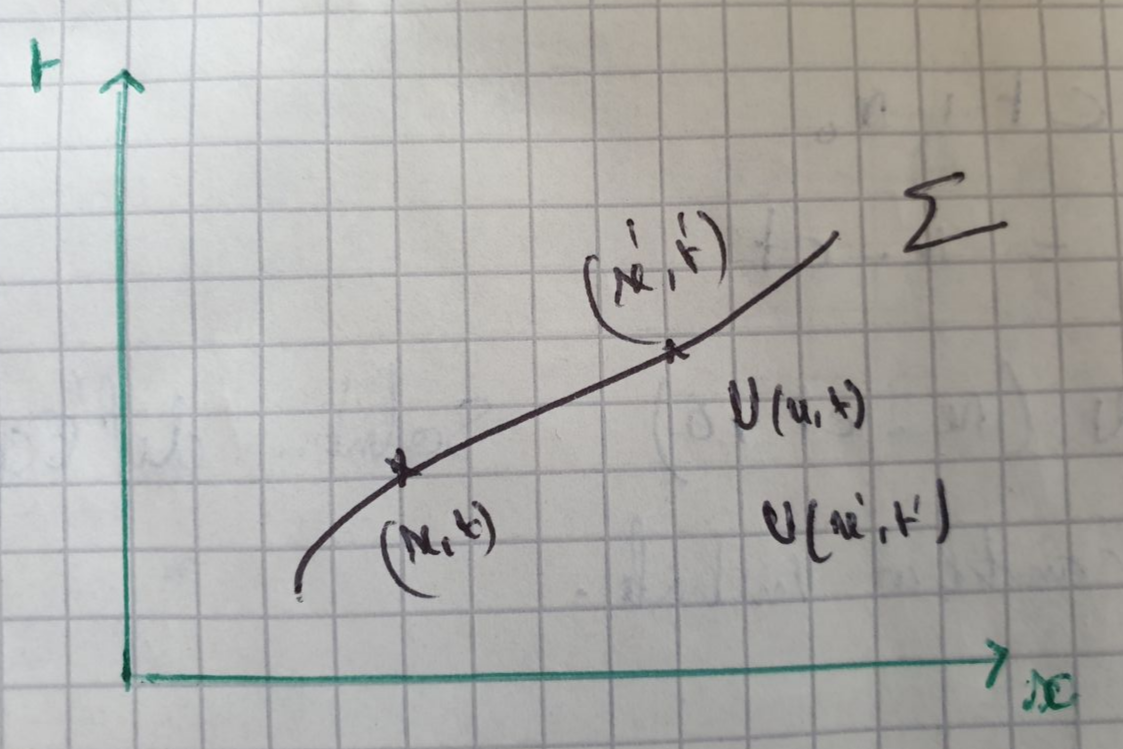
\includegraphics[scale=0.2]{Images_Fichiers/Y1.png}
%\legend{template}
%\label{1CCG}
\end{figure}

Notons $\Sigma$ la courbe du plan param\'etr\'ee par $t\mapsto \left(\begin{array}{c}x(t)\\t\end{array}\right)$ telle que $u$ soit constante le long de $\Sigma$.

La fonction $t\mapsto u(x(t), t)$ est donc constante, donc si tout est r\'egulier sa d\'eriv\'ee exacte en $t$ est nulle :

$$\frac{du(x(t),t)}{dt} = 0$$ 

or la diff\'erentielle de u en $(x(t),t)$ dans la direction $(dx,dt)$ est:

$$ du(x(t),t) = <\nabla u ,(dx,dt)> = \partial_x u(x(t),t)dx+ \partial_t u(x(t), t)dt$$

En divisant cette relation par dt, on obtient :

$$\partial_x u(x(t),t)x'(t)+ \partial_t u(x(t), t)=0$$

Par identification au syst\`eme (1.1), $x'(t)=c$.

Les courbes caract\`eristiques $\Sigma$ sont donc les droites $x(t) = ct+x_0$

On retient $x(t) = ct+x_0$ et $x_0 = x(t)-ct$. 

\begin{figure}[h!]
	\centering 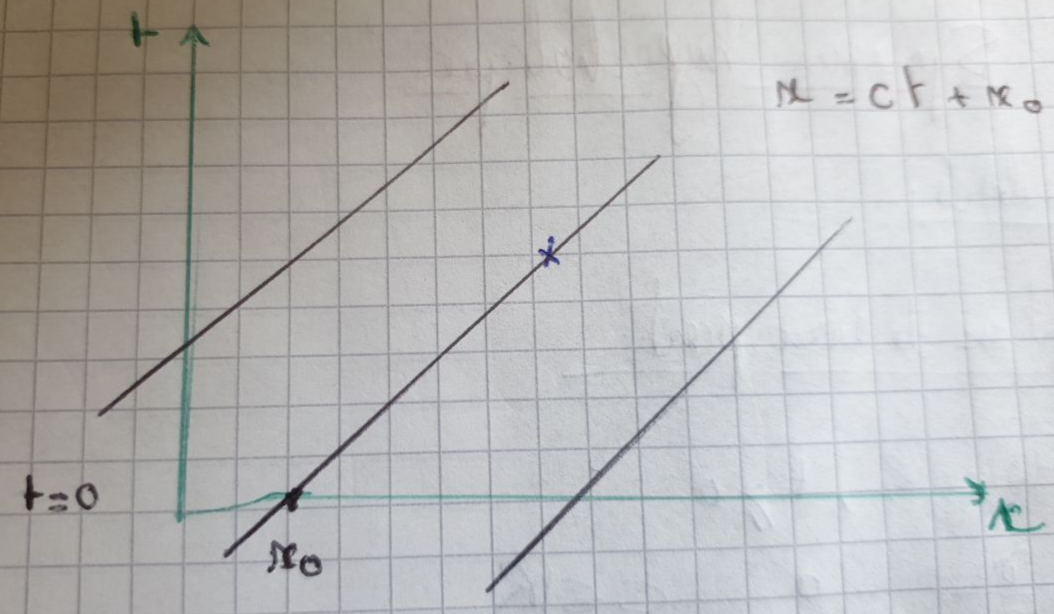
\includegraphics[scale=0.205]{Images_Fichiers/Y2.png}
	\centering 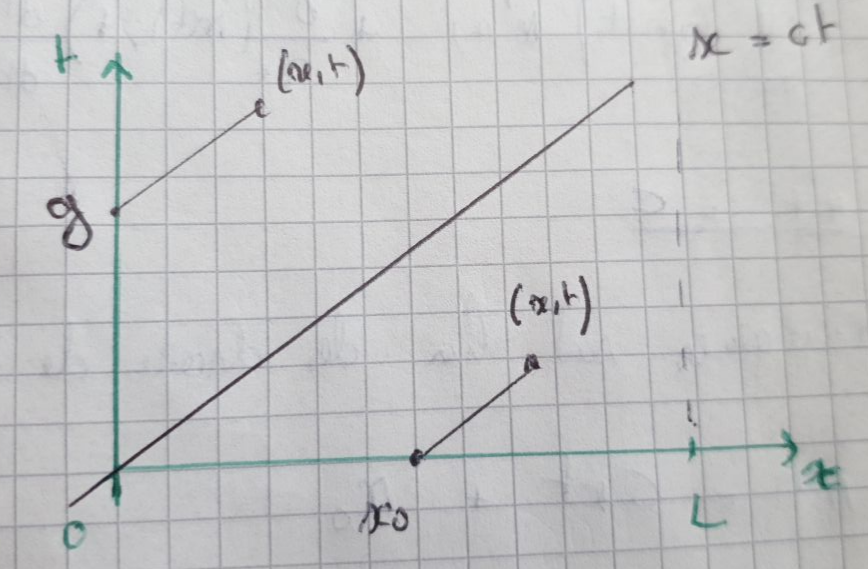
\includegraphics[scale=0.22]{Images_Fichiers/Y3.png}
%\legend{template}
%\label{1CCG}
\end{figure}

\begin{itemize}
\item si $x \geq ct$ : 

Dans ce cas,  $$u(x,t) = u(x_0,0) = u(x - ct,0) = 0$$

d'apr\`es la deuxi\`eme condition initiale.

\item si $x < ct$ :

La courbe caract\'eristique coupe l'axe des ordonn\'ees, donc $$u(x,t) = u\left(0,-\frac{x_0}{c}\right) = e^{\frac{x_0}{c}} = e^{\frac{x}{c} - t}$$ 

d'après la première condition initiale.
\end{itemize}

On a donc au final : \begin{equation}
\label{solution}
u(x,t)=
\left \lbrace \begin{array}{rl}
0 & ~\text{si }  x\geq ct\\
e^{\frac{x}{c}-t} & ~\text{si }  x<ct\\
\end{array}\right.
\end{equation}


\subsection[Cas de c $<$ 0]{\uline{Cas de c $<$ 0:}}

Si $c<0$, On suppose que (1.1) a une solution:

Les droites caract\'eristiques sont inclin\'ees dans l'autre sens et coupe les deux axes. 

On aurait d'une part:
$$u(x,t) =u(ct+x_0, t) = u(x_0, 0) $$

et d'autre part:

$$u(x,t) = u(ct+x_0, t)= u\left(0, -\frac{x_0}{c}\right) $$

Ceci est pr\'esent\'ee dans la figure suivante:

\begin{figure}[h!]
	\centering 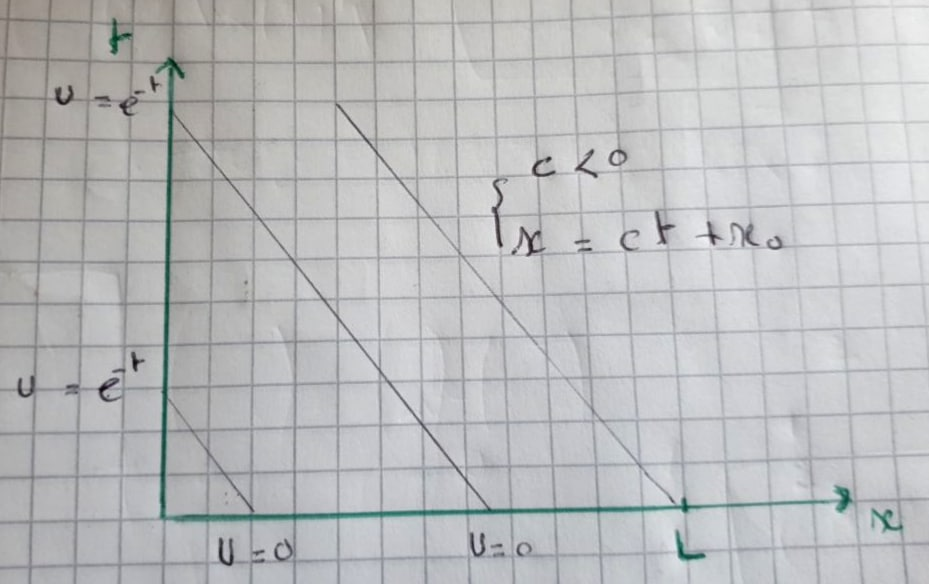
\includegraphics[scale=0.25]{Images_Fichiers/Y4.jpg}
%\legend{template}
%\label{1CCG}
\end{figure}

Donc d'apr\`es les conditions initiales on a:

 $$0=e^{\frac{x_0}{c}}$$
 
ce qui est absurde

Donc si $c<0$, le syst\`eme n'a pas de solution. 


\subsection[La m\'ethode de Godunov]{\uline{La m\'ethode de Godunov:}}
le sh\`ema de Godunov est bas\'e sur la discritisation suivante:

\begin{figure}[h!]
	\centering 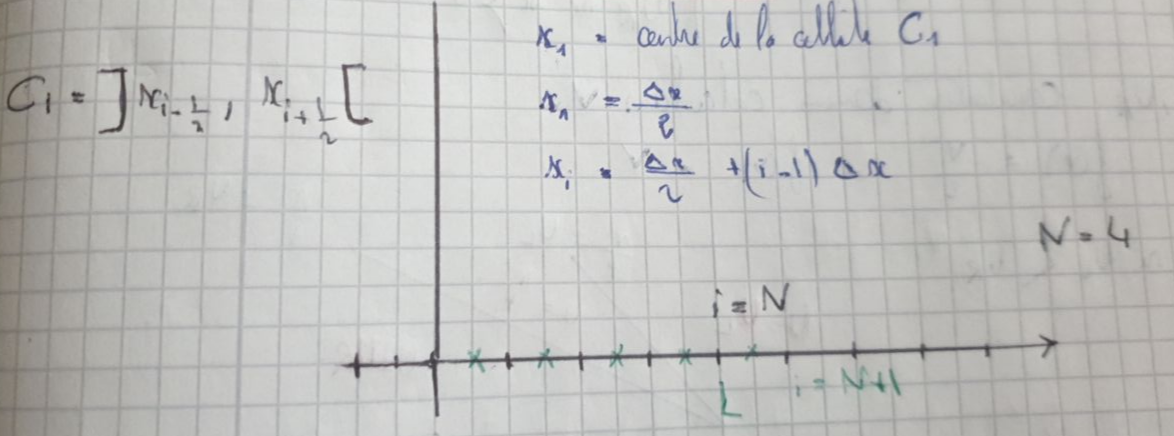
\includegraphics[scale=0.25]{Images_Fichiers/Y5.png}
%\legend{template}
%\label{1CCG}
\end{figure}
avec:
$$u_i^n \sim u(x_i,t_n)$$

Donc (1.1) $\implies$:

$$ \frac {u_i^{n+1} -u_i^n}{\Delta t} + \frac {f(u_{i}^{n},u_{i+1}^{n}) - f(u_{i-1}^{n},u_{i}^{n})}{\Delta x} = 0$$ 
Avec:
$f(u_L, u_R)$ est le flux num\'erique qui repose sur la r\'esolution du probl\`eme de Riemann suivant:
\begin{equation}
\left \lbrace \begin{array}{rl}
\partial_t v +  \partial_x F(v)= 0, & \quad x \in ]0,L[, \; t \in ]0,T[, \\
v(x,0) =
\left \lbrace \begin{array}{rl}
u_L & ~\text{si }  x < 0\\
u_R & ~\text{si }  x>0
\end{array}\right.
\end{array}\right.
\end{equation}

et 

Avec dans notre cas (Transport) $F(u) = cu = u$ (on prend c = 1).

Alors la solution est bas\'ee sur le m\^eme raisonnement qu'en question 1:

\begin{equation}
\label{R}
v(x,t)=
\left \lbrace \begin{array}{rl}
u_R & ~\text{si }  x\geq ct\\
u_L & ~\text{si }  x<ct
\end{array}\right.
\end{equation}

On note $$v(x,t) = R(u_L,u_R,\frac {x}{t})$$

Et on peut en d\'eduire le flux num\'erique par la formule suivante:

$$f(a,b) = F(R(a,b,0))$$

\subsection[Tracer le logarithme de l’erreur en norme $L^1$]{\uline{Tracer le logarithme de l’erreur en norme $L^1$:}}

Pour la validation du code on choisit une  CFL = 0.8 et on visualise la solution et le taux de convergeance pour une valeur de T = 0.5.

\begin{itemize}

\item Solution: 

\begin{figure}[h!]
	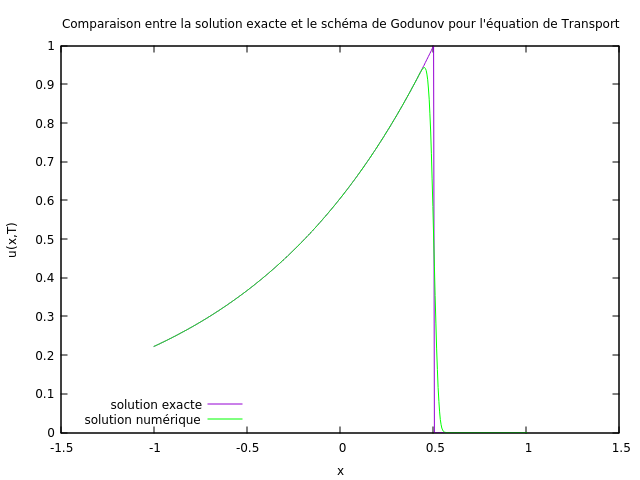
\includegraphics[scale=0.7]{Images_Fichiers/godu1.png}
%\legend{template}
%\label{1CCG}
\end{figure}

\item Erreur:

Voici les résultats obtenus pour différents valeurs de $N$ :
\begin{figure}[h!]
	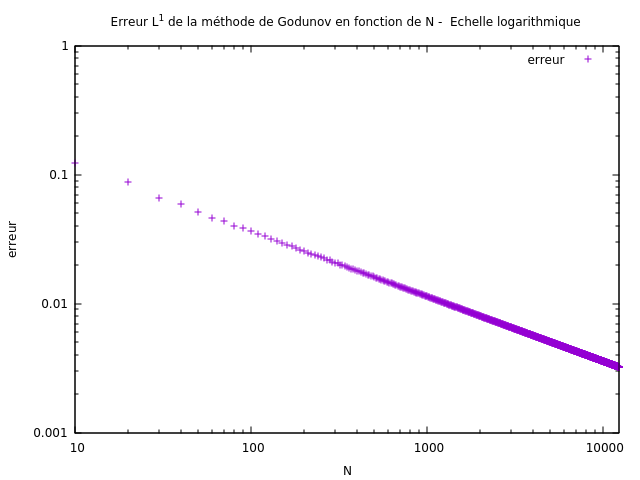
\includegraphics[scale=0.7]{Images_Fichiers/erreur1.png}
%\legend{template}
%\label{1CCG}
\end{figure}


\end{itemize}


Plus N est grand donc le pas $\Delta x$ est petit l'erreur en norme $L^1$ est petite. Ceci est vraie pour plusieurs valeurs de T. 

En partant de la relation th\'eorique de l'erreur en norme $L^1$, on a:

$$erreur(\Delta x) \sim c \times {\Delta x}^{\beta}$$

On peut se permettre de faire l'etude de convergeance en fonction de N (nombre de points) car $\Delta x = \frac{x_{max} - x_{min} }{N}$ 
en effet:

$$erreur(N) \sim c \times N^{-\beta}$$

et en \'echelle logarithmique:

$$ln(erreur(N)) \sim ln(c) -\beta \times ln(N)$$


La pente du graphe en dessus est donc le taux de convergeance pour ce cas de transport. en effet:

$$ \beta = \frac{0.1-0.01}{2\times (0.1-0.01)} =  \frac{1}{2}$$

\subsection[La condition de CFL]{\uline{La condition de CFL:}}
On prend une CFL = 1.1 telle que la condition de stabilit\'e n'est pas v\'erifi\'ee.

Et on a pour c = 1:

$$\frac {\Delta t}{\Delta x } = CFL = 1.1 > 1$$
\newpage
\begin{figure}[h!]
	\centering 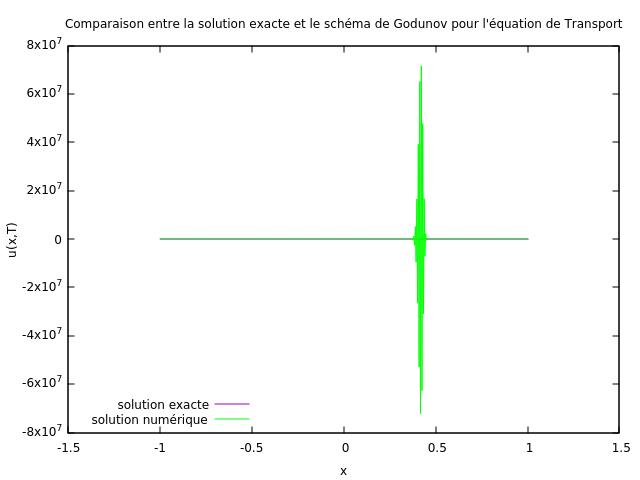
\includegraphics[scale=0.7]{Images_Fichiers/godu2.png}
%\legend{template}
%\label{1CCG}
\end{figure}

Et l'erreur en norme L1 en fonction de N:

\begin{figure}[h!]
	\centering 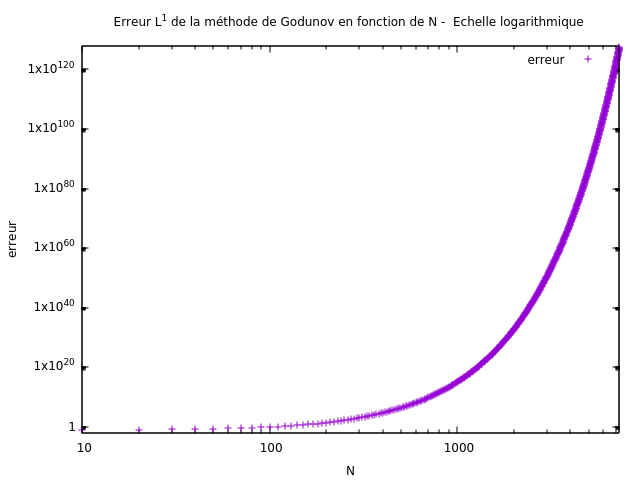
\includegraphics[scale=0.7]{Images_Fichiers/erreur2.png}
%\legend{template}
%\label{1CCG}
\end{figure}

On observe num\'eriquement que le sch\'ema devient instable lorsque la condition de CFL n’est pas satisfaite.

\section[R\`esolution num\'erique de l`\'equation de Burgers]{\uline{R\`esolution num\'erique de l`\'equation de Burgers:}}

Soit maintenant $F(u)=\frac{u^2}{2}$ et on a probl\`eme suivant dit de Burgers \`a r\'esoudre:

\begin{equation}
\label{systeme}
\left \lbrace \begin{array}{rl}
\partial_t u +  \partial_x F(u)= 0, & F(u) = \frac{u^2}{2} \quad x \in ]-1,2[,  \\
u(0,t) = 1, & \; t \in ]0,T[, \\
& u(x,0) =
\left \lbrace \begin{array}{rl}
1 & ~\text{si }  x < 0\\
1-x & ~\text{si }  0 \leq x \leq 1, \\
0 & ~\text{si }  x > 1
\end{array}\right.
\end{array}\right.
\end{equation}

\subsection[La solution de Lax]{\uline{La solution de Lax:}}

On utilise la m\'ethode des caract\'eristiques : 

\begin{figure}[h!]
	\centering 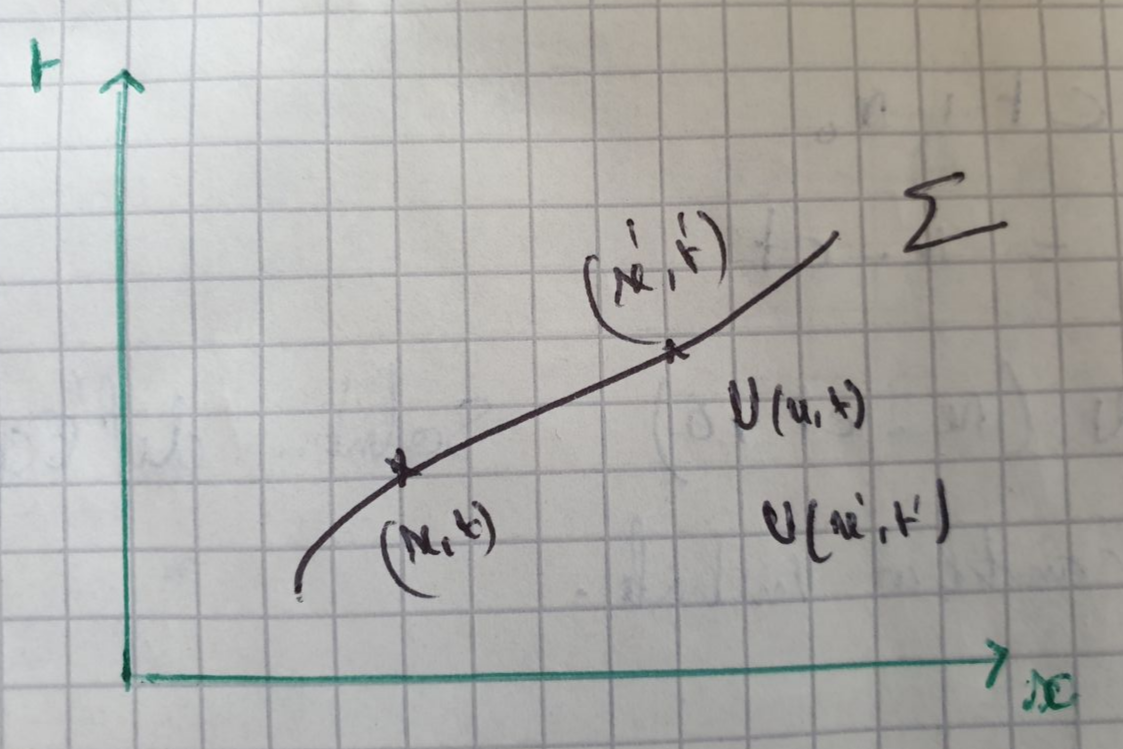
\includegraphics[scale=0.2]{Images_Fichiers/Y1.png}
%\legend{template}
%\label{1CCG}
\end{figure}

Notons $\Sigma$ la courbe du plan param\'etr\'ee par $t\mapsto \left(\begin{array}{c}x(t)\\t\end{array}\right)$ telle que $u$ soit constante le long de $\Sigma$.

La fonction $t\mapsto u(x(t), t)$ est donc constante, donc si tout est r\'egulier sa d\'eriv\'ee exacte en $t$ est nulle :

$$\frac{du(x(t),t)}{dt} = 0$$ 

or la diff\'erentielle de u en $(x(t),t)$ dans la direction $(dx,dt)$ est:

$$ du(x(t),t) = <\nabla u ,(dx,dt)> = \partial_x u(x(t),t)dx+ \partial_t u(x(t), t)dt$$

En divisant cette relation par dt, on obtient :

$$\partial_x u(x(t),t)x'(t)+ \partial_t u(x(t), t)=0$$

Par identification au syst\`eme (1.5), qui peut \^etre r\'e\'ecrit:
$$\partial_t u + F'(u) \partial_x u= 0 \quad avec \; F'(u) = u$$

On a: $$x'(t) = F'(u) = u(x(t),t)$$

Comme $u(x(t),t)$ est constante par d\'efinition de la caract\'eristique.

Donc: $$x'(t) = F'(u) = u(x(t),t)= cst$$

Les courbes caract\`eristiques $\Sigma$ sont donc des droites mais elles ne sont pas forc\'ement parral\`elles.

En effet selon les conditions initiales:

\begin{equation}
\label{systeme}
\left \lbrace \begin{array}{rl}
u(0,t) = 1, & \; t \in ]0,T[, \\
& u(x,0) =
\left \lbrace \begin{array}{rl}
1 & ~\text{si }  x < 0\\
1-x & ~\text{si }  0 \leq x \leq 1, \\
0 & ~\text{si }  x > 1
\end{array}\right.
\end{array}\right.
\end{equation}

Pour calculer des solutions, on a introduit la notion des solutions faibles. Une des solutions faibles est donn\'ee par la vitesse de discontinuit\'e dite vitesse de choc.
$$\sigma = x'(t)$$
La valeur de $\sigma$ doit v\'erifier le crit\`ere de Lax. En effet, un choc de vitesse $\sigma$ s\'eparant les \'etats $u_L$ (\`a gauche) et les \'etats $u_R$ (\`a droite) est admissible au sens de Lax si et seulement si:

$$F'(u_L) > \sigma > F'(u_R)$$

Dans notre cas comme visualis\'e dans la figure en dessous, on pose une courbe de discontinuit\'ee (en rouge) telle que:

$$x(t) = \frac{t}{2} + \frac{1}{2}$$

On retient $$x'(t) = u(x(t),t)$$ et on trace les droites caract\'eristiques.

\begin{figure}[h!]
	\centering 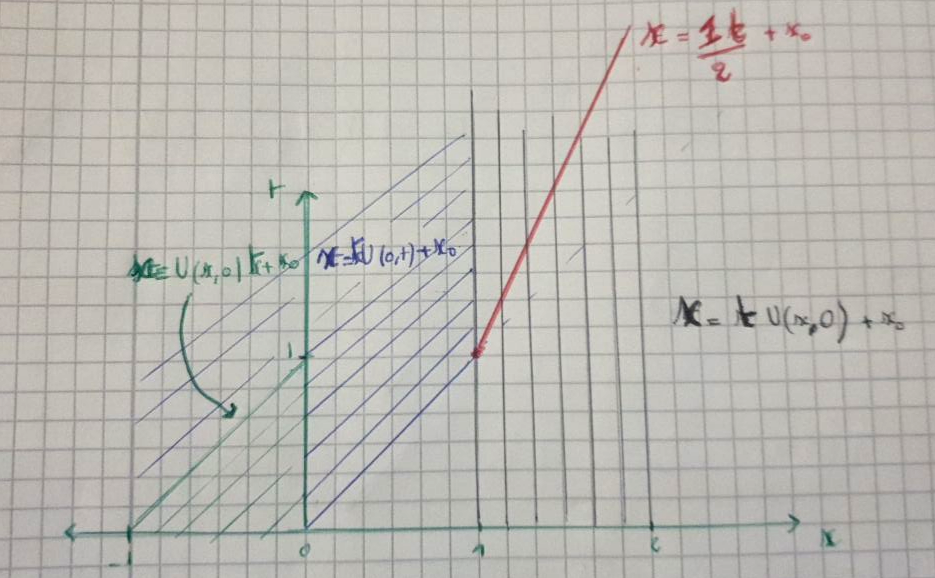
\includegraphics[scale=0.4]{Images_Fichiers/Y6.png}
%\legend{template}
%\label{1CCG}
\end{figure}

en effet, on distingue donc deux cas:
\begin{itemize}

\item cas de choc ou $(t \geq 1)$ : 

Justement pour ce cas on a introduit la droite de discontinuit\'e qui s\'epare deux sous cas.

\begin{equation}
\label{systeme}
u(x,t) =
\left \lbrace \begin{array}{rl}
u_L = 1 & ~\text{si }  x < \frac{t+1}{2}\\
u_R = 0 & ~\text{sinon }  
\end{array}\right.
\end{equation}

On note $u_L$ \`a gauche du choc et $u_R$ \`a droite du choc.

On a $u_L = 1$, $u_R = 0$ et $F'(u) = u$.

Alors selon la relation de Rankine Hugoniot:
$$F(u_R)-F(u_L) = \sigma (u_R-u_L)$$
$$\implies$$
$$\sigma = x'(t) =  \frac{u_L+u_R}{2} = \frac{1}{2}$$

Qui v\'erifie le crit\`ere de Lax:

$$F'(u_L) = u_L = 1 > \sigma = \frac{1}{2} > F'(u_R) = u_R = 0$$

\item  cas sans choc ou $(t < 1)$:

On a dans ce cas trois sous cas d\'efinis selon les conditions initiales.

\begin{itemize}

\item $x <  t$ : 

les caract\'eristiques v\'erifient:
$$x = u(x,t)t + x_0 $$

et coupent soit l'axe des abscisses en $x_0$, soit l'axe des ordonn\'es en $t'$ donc:

$$u(x,t) = u(x_0,0) = u(0,t') = 1$$


\item $x >  1$ : 

les caract\'eristiques v\'erifient:
$$x = u(x,t)t + x_0 $$

et coupent l'axe des abscisses en $x_0$, donc:

$$u(x,t) = u(x_0,0) = 0$$

\item $1 \geq x \geq t$ : 

les caract\'eristiques v\'erifient:
$$x = u(x,t)t + x_0 $$

alors:

$$u(x,t) = u(x_0,0) = 1-x_0$$

Calculons $1-x_0$ en remplacant $u(x,t)$ par $x_0$ dans $x = u(x,t)t + x_0 $ :

On a donc:
$$x = (1-x_0)t + x_0 $$
$\implies$
$$x = (1-x_0)t - (1-x_0) +  1$$
$\implies$
$$x = (1-x_0)(t-1) + 1$$
alors:
$$u(x,t) = u(x_0,0) = 1-x_0 = \frac{x-1}{t-1}$$

\end{itemize}
 

\end{itemize}

On a donc la solution de Lax:

\begin{itemize}

\item $t <  1$ sans choc : 
\begin{equation}
\label{systeme}
 u(x,t) =
\left \lbrace \begin{array}{rl}
\frac{x-1}{t-1} & ~\text{si }  t \geq x \geq 1\\
1 & ~\text{si }  x <  t\\
0 & ~\text{sinon} 
\end{array}\right.
\end{equation}

\item $t \geq  1$ avec choc : 
\begin{equation}
\label{systeme}
u(x,t) =
\left \lbrace \begin{array}{rl}
1 & ~\text{si }  x < \frac{t+1}{2}\\
0 & ~\text{sinon }  
\end{array}\right.
\end{equation}

\end{itemize}


\subsection[le probl\`eme de Riemann pour l`\'equation de Burgers]{\uline{le probl\`eme de Riemann pour l`\'equation de Burgers:}}

Soit le probl\`eme de Riemman pour l`\'equation de Burgers (1.5):
\begin{equation}
\left \lbrace \begin{array}{rl}
\partial_t v +  \partial_x F(v)= 0, & F(v) = \frac{v^2}{2}\\
v(x,0) =
\left \lbrace \begin{array}{rl}
u_L & ~\text{si }  x < 0\\
u_R & ~\text{si }  x>0
\end{array}\right.
\end{array}\right.
\end{equation}

On distingue deux cas posible:

\begin{itemize}

\item si $u_L<u_R$  sans choc : 

\begin{figure}[h!]
	\centering 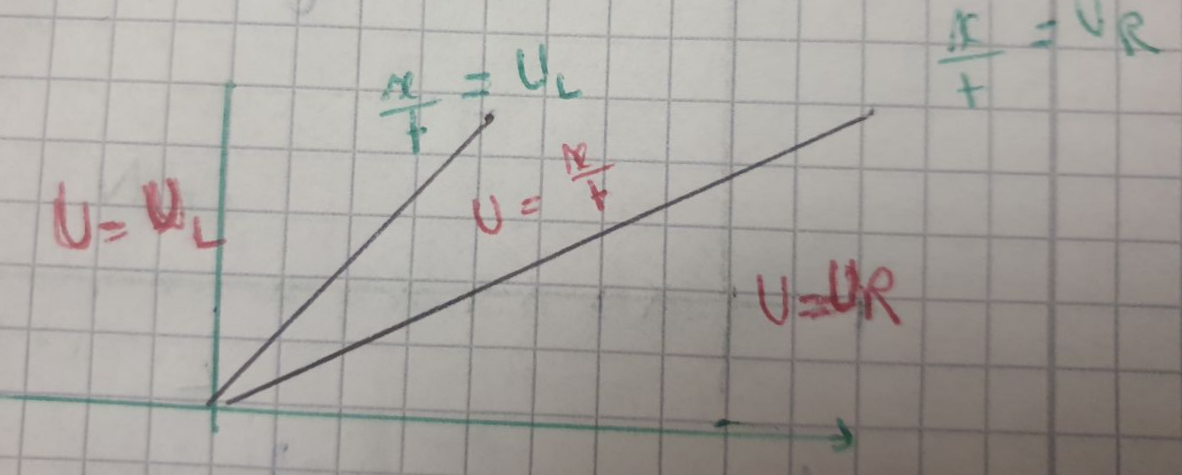
\includegraphics[scale=0.3]{Images_Fichiers/Y7.png}
%\legend{template}
%\label{1CCG}
\end{figure}

\begin{equation}
\label{systeme}
 v(x,t) =
\left \lbrace \begin{array}{rl}
u_L & ~\text{si }  \frac{x}{t} < u_L\\
u_R & ~\text{si }  \frac{x}{t} > u_R\\
\frac{x}{t} & ~\text{sinon} 
\end{array}\right.
\end{equation}

\item si $u_L<u_R$  avec choc : 

Dans ce cas introduit la vitesse de choc donn\'ee par Rankine Hugoniot:

$$\sigma = x'(t) = \frac{u_L + u_R}{2}$$

\begin{figure}[h!]
	\centering 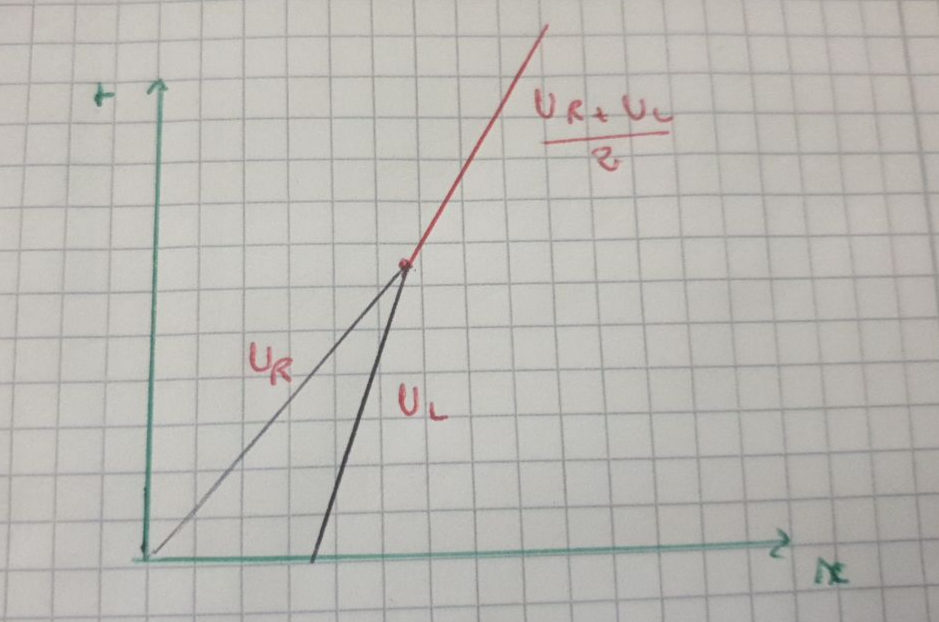
\includegraphics[scale=0.3]{Images_Fichiers/Y8.png}
%\legend{template}
%\label{1CCG}
\end{figure}


\begin{equation}
\label{systeme}
u(x,t) =
\left \lbrace \begin{array}{rl}
u_L & ~\text{si }  \frac{x}{t} < \frac{u_L + u_R}{2}\\
u_R & ~\text{sinon }  
\end{array}\right.
\end{equation}

\end{itemize}

\subsection[La m\'ethode de Godunov]{\uline{La m\'ethode de Godunov:}}

La m\'ethode de Godunov reste la m\^eme sauf que pour le cas de Burgers on adopte les changements:
\begin{itemize}
\item le flux physique:
 $$F(u) = \frac {u^2 }{2}$$
\item le flux num\'erique:

On utilise la solution de Riemman explicit\'ee en dessus en remplacant $\frac{x}{t}$ par 0. Et on note $R(u_L,u_R,0)$:

\begin{itemize}

\item si $u_L<u_R$  sans choc : 

\begin{equation}
\label{systeme}
R(u_L,u_R,0) =
\left \lbrace \begin{array}{rl}
u_L & ~\text{si }  0< u_L\\
u_R & ~\text{si }  0 > u_R\\
\frac{x}{t} & ~\text{sinon} 
\end{array}\right.
\end{equation}

\item si $u_L<u_R$  avec choc : 


\begin{equation}
\label{systeme}
R(u_L,u_R,0) =
\left \lbrace \begin{array}{rl}
u_L & ~\text{si }  0 < \frac{u_L + u_R}{2}\\
u_R & ~\text{sinon }  
\end{array}\right.
\end{equation}

\end{itemize}

avec le flux num\'erque devient:
$$F(R(u_L,u_R,0)) = \frac {R(u_L,u_R,0)^2 }{2}$$

\item La solution exacte: 

On impl\'emente la solution trouv\'e dans la question 1 de la partie Burgers:

\begin{itemize}

\item $t <  1$ sans choc : 
\begin{equation}
\label{systeme}
 u(x,t) =
\left \lbrace \begin{array}{rl}
\frac{x-1}{t-1} & ~\text{si }  t \geq x \geq 1\\
1 & ~\text{si }  x <  t\\
0 & ~\text{sinon} 
\end{array}\right.
\end{equation}

\item $t \geq  1$ avec choc : 
\begin{equation}
\label{systeme}
u(x,t) =
\left \lbrace \begin{array}{rl}
1 & ~\text{si }  x < \frac{t+1}{2}\\
0 & ~\text{sinon }  
\end{array}\right.
\end{equation}

\end{itemize}

\end{itemize}

Pour une CFL = 0.5 et une discretisation de N=100 on a les r\'esultats visualisant la solution et l'erreur $L^1$ en fonction du pas $\Delta x$ en \'echelle logarithmique.

\begin{itemize}

\item Pour $T = 0.5$: 

\begin{itemize}

\item Solution: 

\begin{figure}[h!]
	\centering 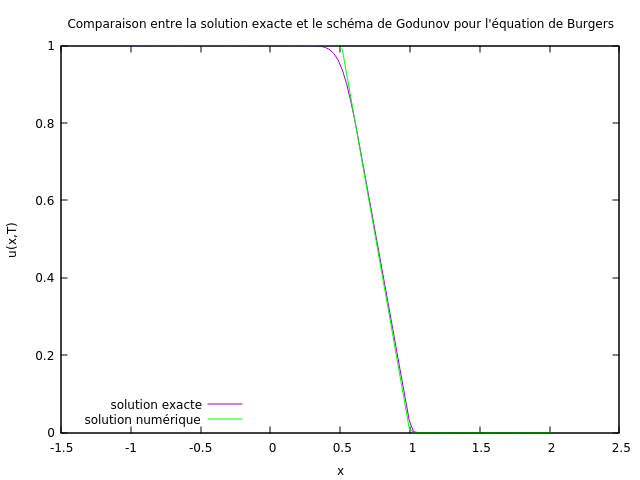
\includegraphics[scale=0.7]{Images_Fichiers/burgers1.png}
%\legend{template}
%\label{1CCG}
\end{figure}
\newpage

\item Erreur $L^1$: 

\begin{figure}[h!]
	\centering 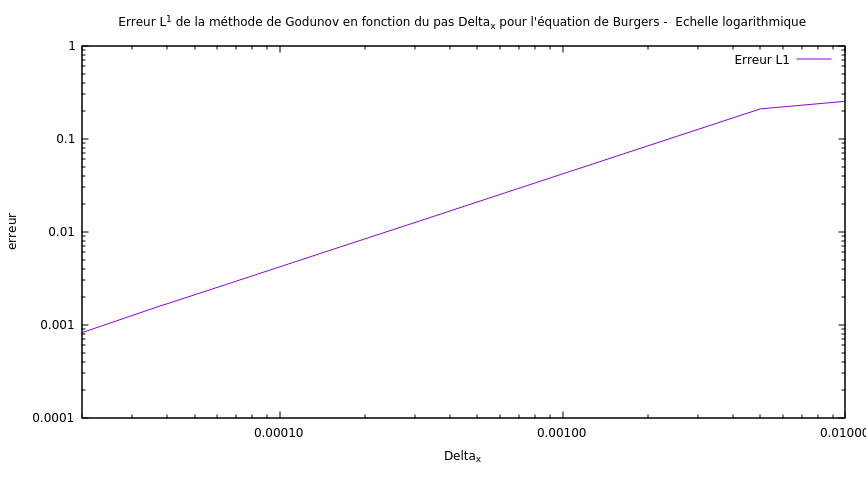
\includegraphics[scale=0.7]{Images_Fichiers/berreur1.png}
%\legend{template}
%\label{1CCG}
\end{figure}

\end{itemize}

\item Pour $T = 1$ : 

\begin{itemize}

\item Solution: 

\begin{figure}[h!]
	\centering 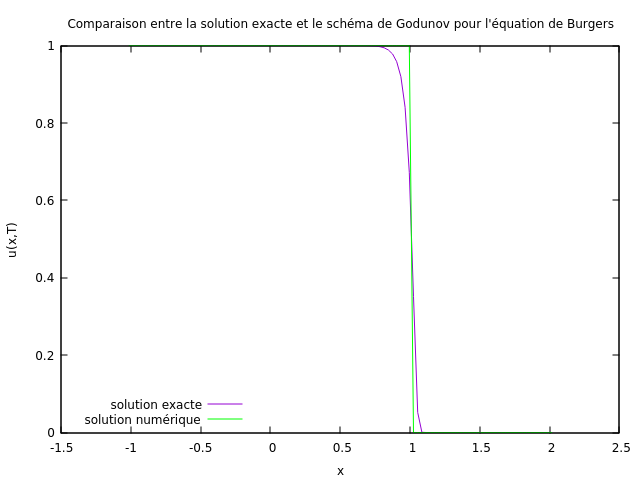
\includegraphics[scale=0.7]{Images_Fichiers/burgers2.png}
%\legend{template}
%\label{1CCG}
\end{figure}

\item Erreur $L^1$: 

\begin{figure}[h!]
	\centering 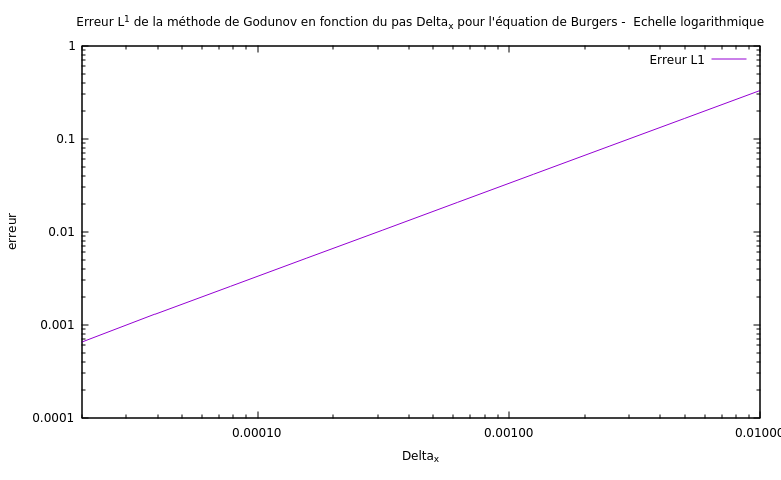
\includegraphics[scale=0.7]{Images_Fichiers/berreur2.png}
%\legend{template}
%\label{1CCG}
\end{figure}

\end{itemize}

\item Pour $T = 2$ : 

\begin{itemize}

\item Solution: 

\begin{figure}[h!]
	\centering 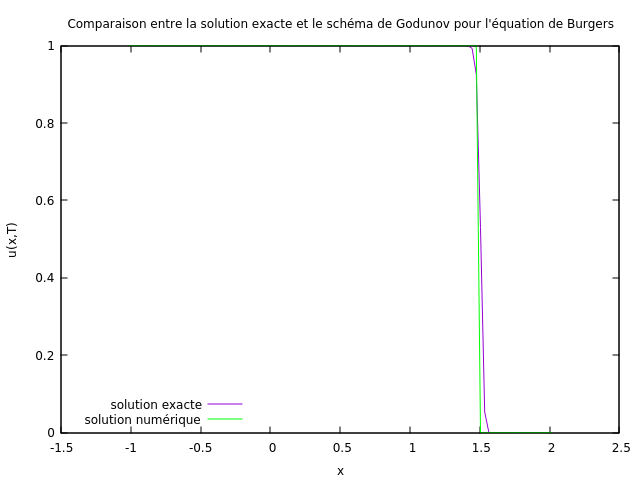
\includegraphics[scale=0.7]{Images_Fichiers/burgers3.png}
%\legend{template}
%\label{1CCG}
\end{figure}

\item Erreur $L^1$: 

\begin{figure}[h!]
	\centering 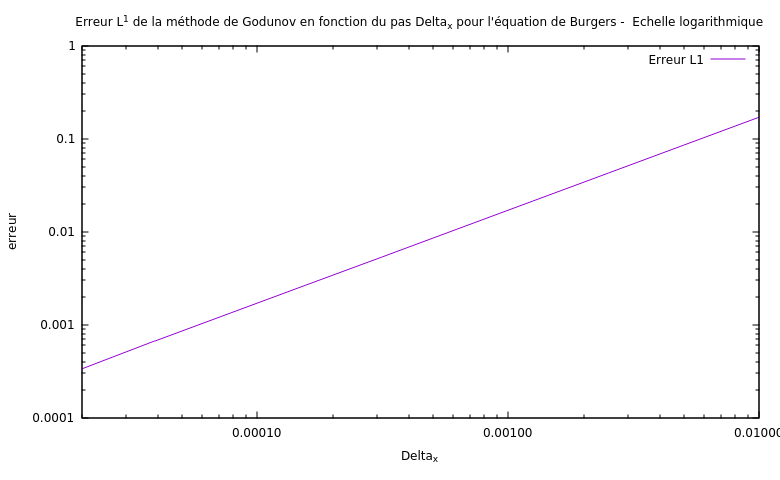
\includegraphics[scale=0.7]{Images_Fichiers/berreur3.png}
%\legend{template}
%\label{1CCG}
\end{figure}

\end{itemize}
\end{itemize}
\newpage
En partant de la relation th\'eorique de l'erreur en norme $L^1$, on a:

$$erreur(\Delta x) \sim c \times {\Delta x}^{\beta}$$

et en \'echelle logarithmique:

$$ln(erreur({\Delta x})) \sim ln(c) + \beta \times ln({\Delta x})$$

La pente des graphes des erreurs en dessus est donc le taux de convergeance pour ce cas de Burgers. en effet:

$$ \beta = \frac{0.00035-0.0001}{0.000035-0.00001} = 1$$


\subsection[La correction MUSCL de van Leer]{\uline{la correction MUSCL de van Leer:}}

le sch\'ema de Muscl en 1D tient en compte l'erreur en $Delta x$ et calcule le flux en $i+ \frac 1 2$. Pour ce, on calcule la pente $s^n_i$ grace au min des modules des pentes (d\'ecentr\'e \`a gauche, \`a droite, centr\'e) et puis on en d\'eduit $r^n_i$ telle que:

$$r_i^n = -f'(w_i^n)s_i^n$$

en effet:

\begin{lstlisting}
double minmod(double a, double b, double c)
{
        double res = 0.0;
        if ((a > 0) && (b > 0) && (c > 0))
        {
                res = a < b ? (a < c ? a : c) : (b < c ? b : c);
        }
        else if ((a < 0) && (b < 0) && (c < 0))
        {
                res = a > b ? (a > c ? a : c) : (b > c ? b : c);
        }
        return res;
}
\end{lstlisting}

et donc:

\begin{lstlisting}
// calcul de pentes
    for (int i = 1; i < gd->N + 1; i++)
    {
        // pour MUSCL
        double a = (gd->un[i] - gd->un[i - 1]) / gd->dx;
        double b = (gd->un[i + 1] - gd->un[i]) / gd->dx;
        double c = (gd->un[i + 1] - gd->un[i - 1]) / 2.0 / gd->dx;

        si[i] = minmod(a,b,c);
        ri[i] = -gd->un[i] * si[i]; // Burgers
     }
\end{lstlisting}        








































